\documentclass[UTF8]{ctexart} 
\usepackage{graphicx} 
\usepackage{hyperref} 
\usepackage{multirow} 
\usepackage{tabularx} 
\usepackage{color} 
\usepackage{textcomp} 
\usepackage{amsmath} 
\usepackage{amssymb} 
\usepackage{amsfonts} 
\usepackage{mathtools} 
\usepackage{enumerate} 
\usepackage{tensor} 
\usepackage{ulem} 
\usepackage{xfrac} 
\usepackage{arydshln} 
% 防御：若不加载 babel 也不至于出错 
\providecommand{\foreignlanguage}[2]{#2} 

\begin{document}
{\centering \textbf{标题}

\par}{\centering 作  者\textsuperscript{1},作  者\textsuperscript{1}

\par}{\centering (1. 作者单位,城市 100000)

\par}\textbf{摘要}：摘要。

\textbf{关键词}：关键词

\textbf{中图分类号}：U455.4             \textbf{文献标识码：}A       \textbf{文章编号：}1000\textendash{}6915(2006)01\textendash{}0001\textendash{}03



{\centering \textbf{TITLE}

\par}{\centering Author\textsuperscript{1}\foreignlanguage{british}{,Author}\textsuperscript{1}

\par}{\centering \textit{(1. Institution\foreignlanguage{british}{,City} 100000\foreignlanguage{british}{,}China)}



\par}\textbf{Abstract}\foreignlanguage{british}{\textbf{：}}Abstract.

\textbf{Key words}\foreignlanguage{british}{：Key words}

\section{一级标题\label{mark-1}}

\subsection{3.1 二级标题}

正文。$In/line=\sum equ\left(at\right)ion$ 

正文。来张{\hyperref[ref-01]{图1}}。

{\centering 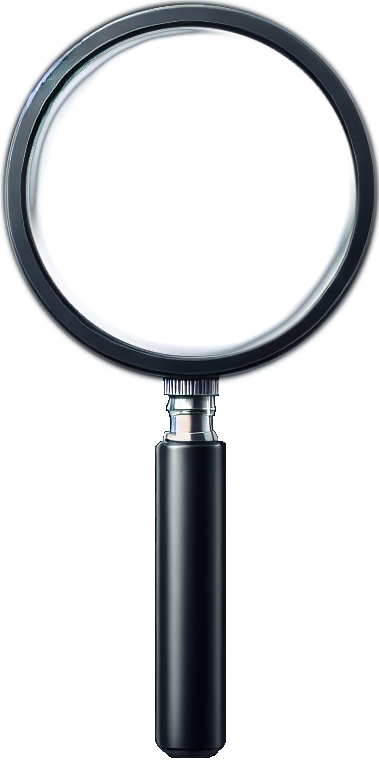
\includegraphics[width=226.75pt]{example_forward.docx.tmp/word/media/image2.png}

\par}{\centering 图1  试验设备\label{ref-01}

\par}{\centering Fig.1  Test equipment

\par}\subsection{3.3 二级标题}

正文\cite{bib1}。看{\hyperref[ref-02]{表1}}。

{\centering 表1  模型及原型材料参数表\label{ref-02}

\par}
\begin{table}
\caption{Table 1  Model and prototype material parameter table}
\begin{tabularx}{\textwidth}{|p{\dimexpr 0.25\linewidth-2\tabcolsep-2\arrayrulewidth}|p{\dimexpr 0.25\linewidth-2\tabcolsep-\arrayrulewidth}|p{\dimexpr 0.25\linewidth-2\tabcolsep-\arrayrulewidth}|p{\dimexpr 0.25\linewidth-2\tabcolsep-\arrayrulewidth}|} \hline 
材料 & \textit{E / }GPa & ${\mu}$ & \textit{d} / mm\\\hline 
C30混凝土 & 24 & 0.2 & 400\\\hline 
工业有机玻璃 & 3.5 & 0.42 & 12\\\hline 
\end{tabularx}
\end{table}
行间公式：
\begin{equation}
\tag{1}
\label{ref-03}\frac{fr}{ac}=\int \limits_{a}^{b}c\mathrm{d}e\pm \sqrt[g]{f}\in \overset{\rightharpoonup }{hij}k\bigcup \limits_{lmn}^{opq}RST\mathit{\alpha }\mathrm{B }\mathit{\chi }\Updelta \iota \mathrm{O }\rho \mathrm{P }
\end{equation}
结论见式{\hyperref[ref-03]{(1)}}。

\section{结  论\label{mark-2}}

结论：

(1)。

\section{参考文献}


\begin{thebibliography}{0}
\bibitem[bib-1]{}{[}1{]}	陈龙, 黄宏伟. 岩石隧道工程风险浅析{[}J{]}. 岩石力学与工程学报, 2005(01): 110～115.
\end{thebibliography}

\bibliographystyle{gbt7714-numerical}

\bibliography{example_forward-bibtex}


\end{document}
